\documentclass[pscyr, nonums]{hedlab}
\usepackage[russian]{babel}
\usepackage[utf8]{inputenc}
\usepackage{graphicx}
\usepackage{listings}

\graphicspath{{images/}}

\lstset{
    basicstyle=\scriptsize,
    inputencoding=utf8,
    extendedchars=\true,
    language=[Sharp]C,
    numbers=left,
    numberstyle=\scriptsize,
    breakatwhitespace=\false,
    breaklines=True,
    tabsize=2,
    keepspaces=true,
}

\labnum{8}
\labname{Создание простых коллекций с помощью PivotViewer}
\student{Голубев А. В.}
\date{}

\begin{document}
    \makeheader
    \emph{Цель работы:} получение общих сведений о технологии PivotViewer, получение практических навыков в создании коллекций с помощью PivotViewer.

    \emph{Задачи:}
    \begin{enumerate}\itemsep-5pt
        \item Установить PivotViewer Excel Tool for Pivot Collection
        \item Создать коллекцию с помощью Excel Tool for Pivot Collection
        \item Опубликовать коллекцию в Silverlight-форме
    \end{enumerate}

    \emph{Скриншоты:}
    \begin{figure}[ht]
        \center
        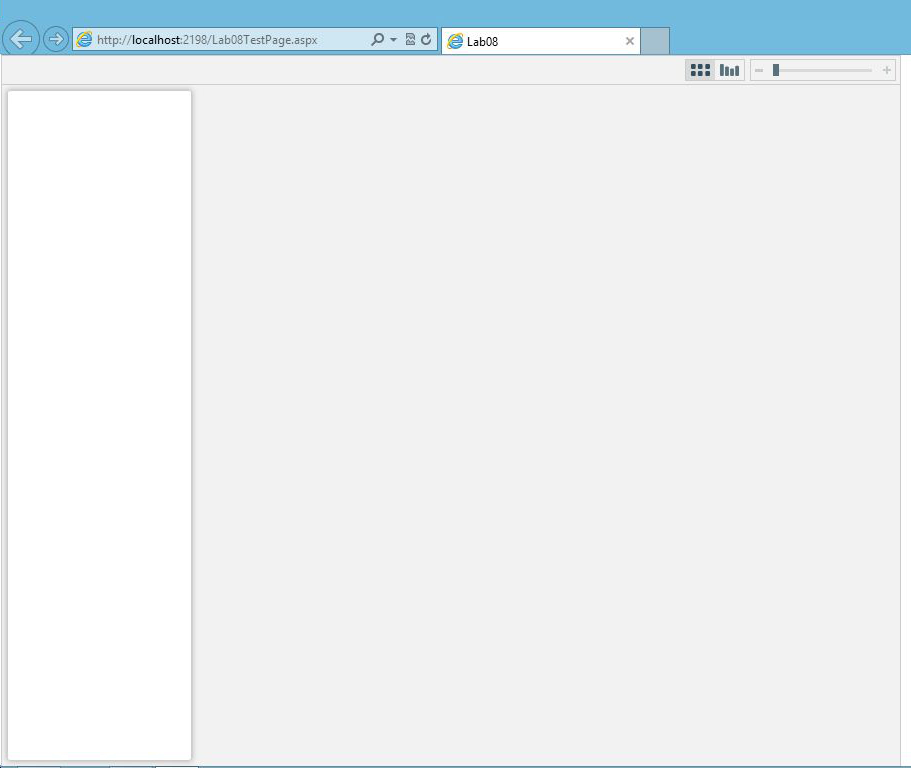
\includegraphics[width=0.9\textwidth]{Lab08_01}
        \caption{Главная страница с Silverlight-формой}
    \end{figure}

    \pagebreak

    \emph{Исходный код:}
    \begin{center}
        \textbf{Главная страница}
    \end{center}
    \lstinputlisting{./source/MainPage.xaml.cs}

    \begin{center}
        \textbf{Разметка главной страницы}
    \end{center}
    \lstinputlisting{./source/MainPage.xaml}
\end{document}
